\documentclass{article}
\usepackage[left=2cm,right=2cm,top=2cm,bottom=2cm]{geometry}
\usepackage[utf8]{inputenc}
\usepackage[german]{babel}
\usepackage{amsmath}
\usepackage{dsfont}
\usepackage[export]{adjustbox}
\usepackage{amsthm}
\usepackage{color}
\usepackage{amsfonts}
\usepackage{amssymb}
\usepackage{wasysym}
\usepackage{makeidx}
\usepackage{graphicx}
\usepackage[colorlinks=true,urlcolor=blue,linkcolor=blue]{hyperref}
\usepackage{ziffer}
\usepackage{minted}
\usepackage{xcolor}
\usepackage{framed}
\usepackage{mdframed}
\usepackage{subfiles}
\usemintedstyle{emacs}

\definecolor{purp}{HTML}{9A72AC}
\definecolor{re}{HTML}{FC6255}
\definecolor{gre}{HTML}{83C167}
\definecolor{blu}{HTML}{58C4DD}
\definecolor{shadecolor}{rgb}{0.85,0.85,0.85}
\definecolor{bg}{rgb}{0.95,0.95,0.95}
\setlength{\parindent}{0em} 

\BeforeBeginEnvironment{minted}{\begin{mdframed}[linewidth =2 ,backgroundcolor=bg , linecolor=black, linewidth=0.5]}
\AfterEndEnvironment{minted}{\end{mdframed}}

\newtheorem{defi}{Definition}
\BeforeBeginEnvironment{defi}{\begin{mdframed}[linewidth =2 ,backgroundcolor=bg , linecolor=black, linewidth=0.5]}
\AfterEndEnvironment{defi}{\end{mdframed}}

\newcommand{\bsp}{\textbf{Beispiel}:}
%\newcommand{\task}{\textbf{Aufgabe}:}

\newcommand{\bol}[1]{\textbf{#1}}
\newcommand{\q}[1]{\glqq #1\grqq}
\newcommand{\DODO}[1]{\textbf{\textcolor{red}{DODO:}} #1 \\ \begin{center}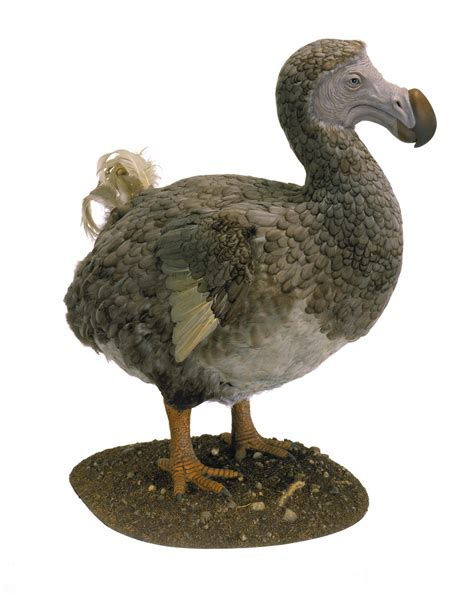
\includegraphics[scale=0.2]{../../media/dodo.jpg} \end{center}}

\newenvironment{task}[1]{
    \begin{shaded*}
    \textbf{Aufgabe #1}:
}{
    \end{shaded*}
}

\begin{document}
Dem aufmerksamen Leser dieses Skripts ist sicher aufgefallen, dass in vielen Fällen von der Warteschlange die Rede war, jedoch die Implementierungen meistens mit einer Form von Liste benannt waren. Das liegt daran, dass mit der Erweiterung der Funktionalität der Listen die reine Form der Warteschlange \q{zerstört} wurde. \\ 
Man unterscheidet in der Informatik im Wesentlichen drei Formen von Listen (natürlich gibt es auch davon noch weitere Untertypen bzw. verschiedene Implementierungsweisen).
\begin{enumerate}
    \item \textbf{Warteschlange}: das zuerst angefügte Element verlässt die Liste auch zuerst (First-In-First-Out: FIFO-Prinzip)
    \item \textbf{Stack}: das zuletzt angefügte Element verlässt die Liste zuerst (Last-In-First-Out: LIFO-Prinzip)
    \item \textbf{Sortierte Liste}: ein Element wird gemäß einer bestimmten vorgegebenen Logik in die Liste eingefügt. Es wird in der Regel nicht exklusiv von vorne oder von hinten entfernt.
\end{enumerate}
Durch die Erweiterung der Funktionalität der Feld-Liste haben wir also beispielsweise die Warteschlange mit der sortierten Liste vermischt. Die Experten haben dies auch für die verkettete Liste in Aufgabe 8 aus dem letzten Kapitel bereits durchgeführt. \\
Es wäre ungeschickt die verkettete Liste die Warteschlange, den Stack und die sortierte Liste jeweils einzeln vollständig zu implementieren. Viele Methoden überschneiden sich in ihrer Funktionalität bzw. sind vollständig identisch. Klüger wäre also, die gesamte Logik aller Listen in einer Struktur (z.B. MeineListe, MyList) zusammenzufassen und dann für die Warteschlange, den Stack oder die sortierte Liste nur die Methoden der Liste zu übernehmen, die für diesen Fall Anwendung finden. \\
Man spricht hier von einer \textbf{Adapter-Klasse}, da keine neue Logik hinzugefügt wird, sondern nur auf die Funktionalität einer bereits bestehenden Klasse zugegriffen wird. \\
\vspace{2mm}
Bevor wir eine allgemeine Listen-Klasse erstellen und die Adapterklassen definieren, muss noch der Stack und die sortierte Liste untersucht werden.

\subsection{Stack}

Ein Stack entspricht einem Stapel in der \q{realen} Welt recht genau. Eine hilfreiche Vorstellung ist ein hoher Bücherstapel, bei dem nur das zuletzt hinzugefügt Buch, nämlich das Oberste, ungefährdet wieder entfernt werden können. Gehen wir von einer Implementierung mit Kompositum aus, könnte eine Folge von Einfüge- bzw. Entfernungsoperatoren wie folgt aussehen: 
\begin{center}
    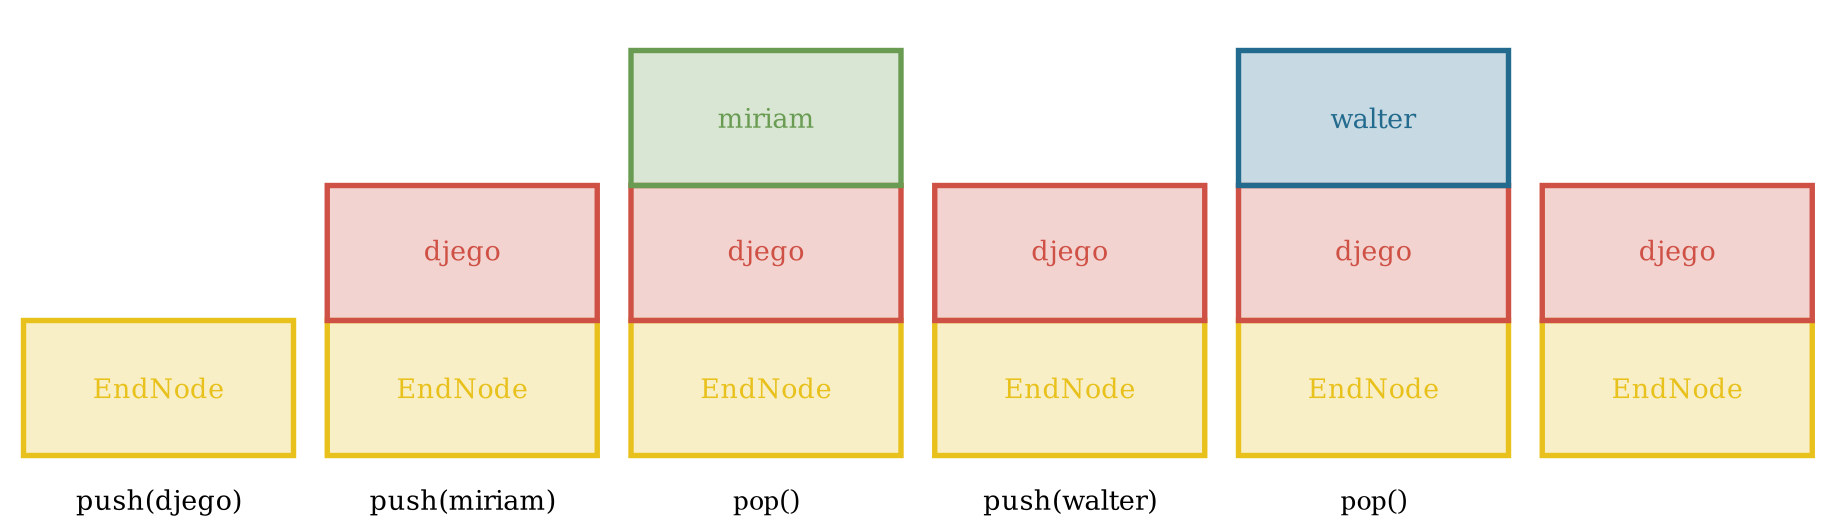
\includegraphics[scale=0.25]{../../media/stack.png}
\end{center}
Stacks werden in der Informatik häufig verwendet, sie spielen z.B. eine Rolle bei Tiefendurchläufen von Graphen (siehe 11|2) und sind ein Hilfsmittel zur Syntaxüberprüfung, bzw. zur Auswertung von Ausdrücken allgemein. (siehe auch formale Sprachen 12|1). \\
Auch beim Ausführen von Methoden werden die noch abzuwarbeitenden Anwendungen auf einem Stack verwaltet. So kommt es bei rekursiven Methoden auch dazu, dass zuerst bis zur \q{tiefsten Stelle} vorgedrungen wird, da immer mehr Aufrufe auf den Stack gelegt werden, bis an der Abbruchbedingung schließlich einer fertiggestellt wird und es zurück nach unten geht. \\
\textit{Hinweis:} Hat man eine rekursive Methode, die keine Abbruchbedingung hat, so wird das Programm abgebrochen, sobald der Befehlsstack vollgelaufen ist (er hat also eine begrenzte Größe). So wird eine Endlosschleife vermieden. \\
Im Gegensatz zur Warteschlange wird bei einem Stack immer vorne eingefügt, anstatt hinten (in beiden Implementierungen heißt die Methode im Englischen push()). Das Entfernen verläuft völlig analog zur Warteschlange.

\subsection{Sortierte Listen}
Im dritten Kapitel und im fünften Kapitel haben die Experten sich bereits mit Sortierung beschäftigt. Die wichtigste Voraussetzung, um überhaupt sortieren zu können, ist eine Vorschrift was \q{größer} bzw. \q{kleiner} ist. Im Falle der Menschen wurde willkürlich das Alter ausgewählt, es hätte aber auch der Name oder eine Kombination aus beidem als Schlüssel zur Sortierung dienen können. Als Festlegung gehen wir von einer aufsteigend sortierten Liste aus. \\
Für die Implementierung gehen wir wieder von einer verketteten Liste mit Kompositum aus. Die Listenklasse muss dann lediglich wieder das Anfügen starten: 
\begin{minted}{Java}
    //class MyListComp
    public void appendSorted(DataElement data) {
        root = root.appendSorted(data);
    }

    //class Node 
    public abstract Node appendSorted(DataElement data);

    //class DataNode 
    public Node appendSorted(DataElement data) {
        if(this.data.isGreater(data)) {
            return new DataNode(this, data);
        }
        next = next.appendSorted(data);
        return this;
    }

    //class EndNode
    public Node appendSorted(DataElement data){
        return new DataNode(this, data);
    }
\end{minted}
Jeder Datenknoten prüft, ob seine Daten größer sind als die einzufügenden, denn dann muss ein neuer Datenknoten geschaffen werden und dem Vorgänger als neuer Nachfolger übergeben werden. Der aktuelle Datenknoten setzt sich selbst dann als Nachfolger des neuen Knotens. \\
\begin{center}
    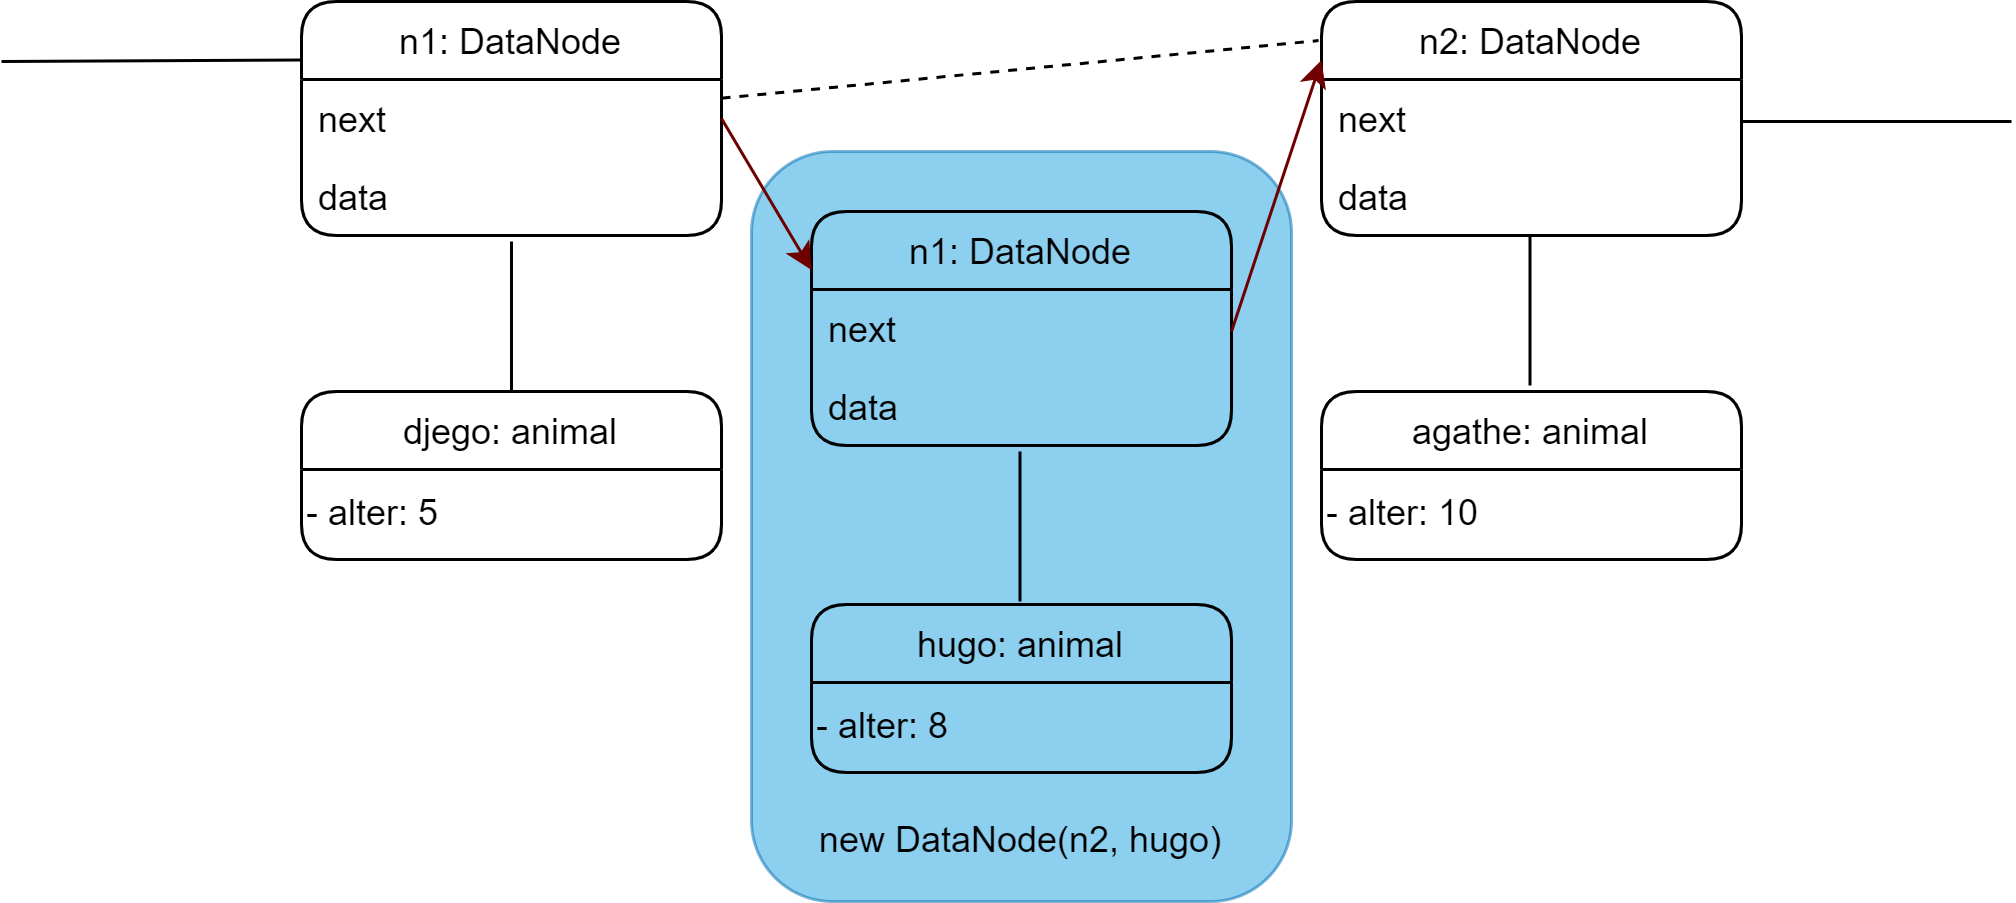
\includegraphics[scale=0.2]{../../media/append_sorted_objects.png}   
\end{center}
Das gleiche geschieht im Endknoten, allerdings in jedem Fall, da der neue Knoten das größte Element enthalten muss, wenn es bis ganz nach hinten \q{durchgekommen} ist.

\subsection{Die Adapter-Klassen}
Mit Hilfe dieser Vorarbeit ist jetzt alles geklärt, um das letzte große Projekt in Angriff zu gehen, die Implementierung der Liste mit allen drei Adapterklassen. \\
Die Listen-Klasse soll dabei alle Logik enthalten, ein Auszug des Klassendiagramms sieht wie folgt aus:
\begin{center}
    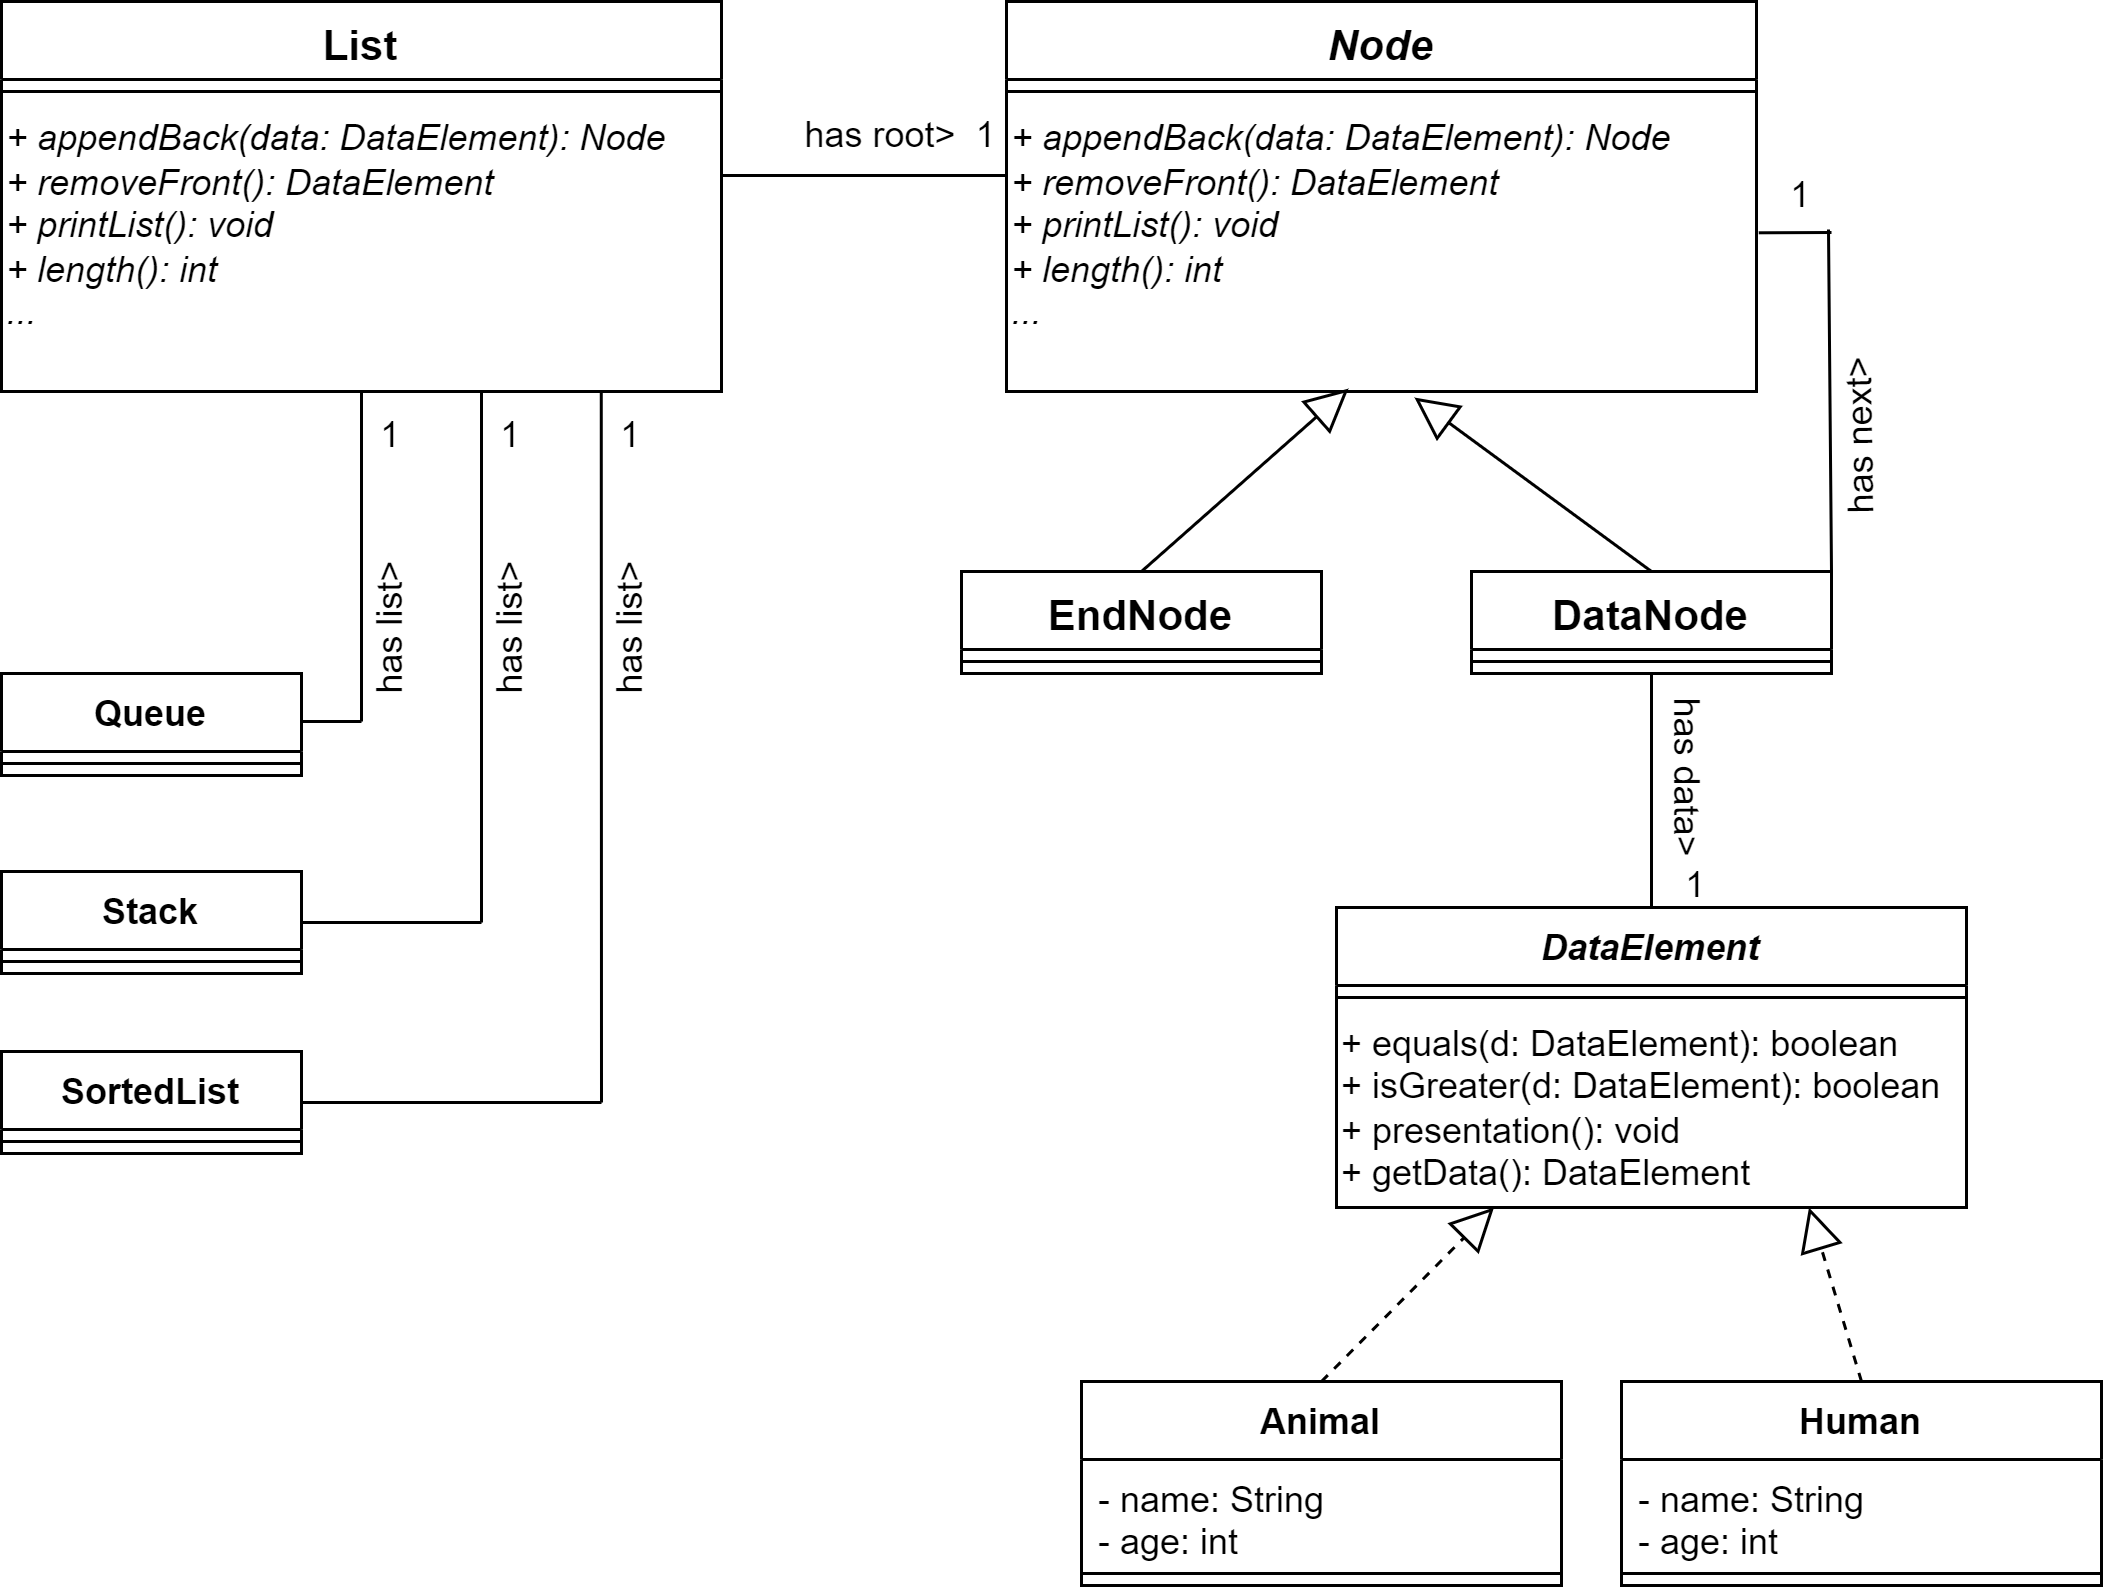
\includegraphics[scale=0.2]{../../media/adapter_lists.png}   
\end{center}
\begin{task}{Abschlussaufgabe}
Implementieren Sie die obige Struktur, insbesondere die Adapterklassen. Erweitern Sie dazu sukzessive die Methoden in der Klasse Liste. Sie können auf bisherige Implementierungen zurückgreifen. 
\end{task}
Für Interessierte gibt es auch am Ende dieses Kapitels noch mehr zu entdecken, einige Anregungen: 
\begin{itemize}
    \item Untersuchen Sie die Java-Klasse ArrayList und LinkedList, vergleichen Sie mit unserer eigenen Implementierung.
    \item \textbf{Generics}: Auch Java bietet bereits die Möglichkeit allgemeinere Listen zu definieren, so gibt kann eine ArrayList eine Liste von Strings oder Zahlen oder anderen Objekten sein, recherchieren Sie die Funktionsweise.
\end{itemize}
\end{document}